\documentclass{article}
\usepackage{geometry}[a4paper, left=20mm, top=20mm]
\usepackage{authblk}
\usepackage{enumitem}
\usepackage{amsmath}
\usepackage{tikz}
\tikzstyle{vertex}=[circle, draw=black, fill=black, inner sep=0pt,
minimum size=4pt]
\usepackage{hyperref}
\hypersetup{
  colorlinks=true,
  urlcolor=magenta,
}

\title{\texttt{Semigroups} --- Zero to Hero --- Worksheet}

\author[1]{James Mitchell}
\author[2]{Reinis Cirpons}
\author[1]{Joseph Edwards}

\affil[1]{University of St Andrews}
\affil[2]{Nantes Université, École Centrale Nantes, CNRS, Inria,
LS2N, UMR 6004, France}

\date{May 2026}

\begin{document}
\maketitle

This worksheet contains some exercises to be completed in \texttt{GAP} with the
use of the \texttt{Semigroups} package as part of the GAP workshop session of
NBSAN 40. The problems have been written in a deliberately terse way to
encourage attendees to experiment with the package and explore its associated
manual:
\url{https://semigroups.github.io/Semigroups/doc/chap0_mj.html}.

As well as inspecting the package manual, please also feel free to ask questions
to James, Reinis or Joe!

\begin{enumerate}
  \item Let $J_n$ denote the Jones monoid of degree $n$, and
    \[
      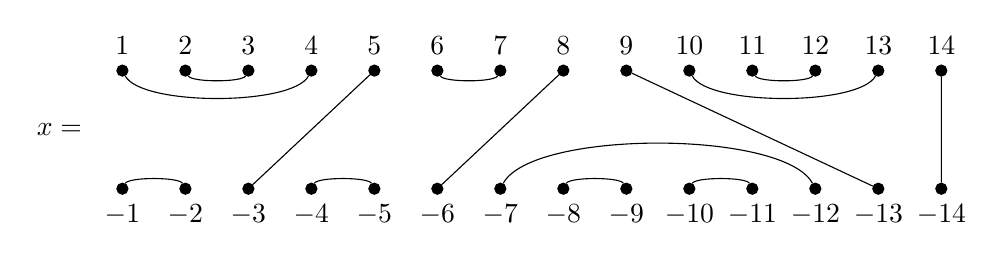
\begin{tikzpicture}[xscale=0.8, yscale=1.5]
  % Label
  \node at (0, 0) {$x=$};

  % Top Nodes
  \node (1) at (1, 0.5) [vertex, label=above:$1$]{};
  \node (2) at (2, 0.5) [vertex, label=above:$2$]{};
  \node (3) at (3, 0.5) [vertex, label=above:$3$]{};
  \node (4) at (4, 0.5) [vertex, label=above:$4$]{};
  \node (5) at (5, 0.5) [vertex, label=above:$5$]{};
  \node (6) at (6, 0.5) [vertex, label=above:$6$]{};
  \node (7) at (7, 0.5) [vertex, label=above:$7$]{};
  \node (8) at (8, 0.5) [vertex, label=above:$8$]{};
  \node (9) at (9, 0.5) [vertex, label=above:$9$]{};
  \node (10) at (10, 0.5) [vertex, label=above:$10$]{};
  \node (11) at (11, 0.5) [vertex, label=above:$11$]{};
  \node (12) at (12, 0.5) [vertex, label=above:$12$]{};
  \node (13) at (13, 0.5) [vertex, label=above:$13$]{};
  \node (14) at (14, 0.5) [vertex, label=above:$14$]{};

  % Bottom Nodes
  \node (1') at (1, -0.5) [vertex, label=below:$-1$]{};
  \node (2') at (2, -0.5) [vertex, label=below:$-2$]{};
  \node (3') at (3, -0.5) [vertex, label=below:$-3$]{};
  \node (4') at (4, -0.5) [vertex, label=below:$-4$]{};
  \node (5') at (5, -0.5) [vertex, label=below:$-5$]{};
  \node (6') at (6, -0.5) [vertex, label=below:$-6$]{};
  \node (7') at (7, -0.5) [vertex, label=below:$-7$]{};
  \node (8') at (8, -0.5) [vertex, label=below:$-8$]{};
  \node (9') at (9, -0.5) [vertex, label=below:$-9$]{};
  \node (10') at (10, -0.5) [vertex, label=below:$-10$]{};
  \node (11') at (11, -0.5) [vertex, label=below:$-11$]{};
  \node (12') at (12, -0.5) [vertex, label=below:$-12$]{};
  \node (13') at (13, -0.5) [vertex, label=below:$-13$]{};
  \node (14') at (14, -0.5) [vertex, label=below:$-14$]{};

  % Top Edges
  \draw (1) .. controls +(0.3,-0.3) and +(-0.3,-0.3) .. (4);
  \draw (2) .. controls +(0.1,-0.1) and +(-0.1,-0.1) .. (3);
  \draw (6) .. controls +(0.1,-0.1) and +(-0.1,-0.1) .. (7);
  \draw (10) .. controls +(0.3,-0.3) and +(-0.3,-0.3) .. (13);
  \draw (11) .. controls +(0.1,-0.1) and +(-0.1,-0.1) .. (12);

  % Bottom Edges
  \draw (1') .. controls +(0.1,0.1) and +(-0.1,0.1) .. (2');
  \draw (4') .. controls +(0.1,0.1) and +(-0.1,0.1) .. (5');
  \draw (7') .. controls +(0.5,0.5) and +(-0.5,0.5) .. (12');
  \draw (8') .. controls +(0.1,0.1) and +(-0.1,0.1) .. (9');
  \draw (10') .. controls +(0.1,0.1) and +(-0.1,0.1) .. (11');

  % Transverse edges
  \draw (5) to (3');
  \draw (8) to (6');
  \draw (9) to (13');
  \draw (14) to (14');
\end{tikzpicture}
    \]
    \begin{enumerate}
      \item How many elements does $J_{14}$ contain?
      \item How many idempotent elements does $J_{14}$ contain?
      \item How many idempotent elements does the Green's
        $\mathcal{D}$-class of $x$ in $J_{14}$ contain?
      \item How many idempotent elements with $7$ in the domain does
        the Green's $\mathcal{D}$-class of $x$ in $J_{14}$ contain?
    \end{enumerate}
\end{enumerate}

\end{document}
